%This work is licensed under the Creative Commons
%Attribution-ShareAlike 4.0 International License. To view a copy of
%this license, visit http://creativecommons.org/licenses/by-sa/4.0/ or
%send a letter to Creative Commons, PO Box 1866, Mountain View, CA
%94042, USA.

%This work is licensed under the Creative Commons
%Attribution-ShareAlike 4.0 International License. To view a copy of
%this license, visit http://creativecommons.org/licenses/by-sa/4.0/ or
%send a letter to Creative Commons, PO Box 1866, Mountain View, CA
%94042, USA.

%\documentclass[gray,handout, pdftex, 11pt]{beamer}
%\documentclass[handout, pdftex, 11pt]{beamer}

\documentclass[pdftex, 11pt]{beamer}

\usepackage[utf8]{inputenc}
\usepackage[T1]{fontenc}
\usepackage{lmodern}
%\usepackage[italian]{babel}
\usepackage{graphicx}
\usepackage{listings}
\usepackage{microtype}
\usepackage{acronym}
\usepackage{array}
\usepackage{tikz}
\usetikzlibrary{shapes, chains, scopes, shadows, positioning, arrows,
  decorations.pathmorphing, calc}

\colorlet{c1}{green!20}
\colorlet{c2}{blue!10}
\colorlet{drawColor}{black!50}
\colorlet{commentColor}{green!70!black!90}

\tikzstyle{oval}=[ellipse, align=center, drop shadow, draw=drawColor, fill=white]
\tikzstyle{rect}=[rectangle, rounded corners=2pt, align=center, drop
shadow, draw=drawColor, fill=white]
\tikzstyle{comment}=[text=commentColor,font=\itshape]
\tikzstyle{textLab}=[]
\tikzstyle{arrow}=[->, very thick, >=stealth', draw=black!80]
\tikzstyle{darrow}=[->, dash pattern=on 3pt off2pt, very thick, >=stealth', draw=black!80]
\tikzstyle{fStartEnd}=[ellipse, align=center, drop shadow, draw=drawColor, fill=white]
\tikzstyle{fInput}=[trapezium, trapezium left angle=70, trapezium right angle=110,
align=center, drop shadow, draw=drawColor, fill=white]
\tikzstyle{fProcess}=[rectangle, align=center, drop shadow, draw=drawColor, fill=white]
\tikzstyle{fSelection}=[diamond, shape aspect=3, align=center, drop
shadow, draw=drawColor, fill=white]
\tikzstyle{fOutput}=[tape, tape bend top=none, align=center, drop shadow, draw=drawColor, fill=white]
\tikzstyle{mem}=[rectangle, align=center, draw=drawColor, fill=white]
\tikzstyle{clo}=[cloud, aspect=2, align=center, drop shadow, draw=drawColor, fill=white]

\lstdefinestyle{customc}{
   language=C,
   % basicstyle=\small\ttfamily\bfseries,
   basicstyle=\ttfamily,
   keywordstyle=\color{blue}\ttfamily,
   stringstyle=\color{red}\ttfamily,
   commentstyle=\color{green}\ttfamily,
   morecomment=[l][\color{magenta}]{\#},
   % breaklines=false,
    breaklines=true, breakatwhitespace=false,
   frameround=fttt,
   frame=trBL,
   backgroundcolor=\color{yellow!20},
   numbers=left,
   stepnumber=1,    
   firstnumber=1,
   numberfirstline=true,
   numberstyle=\tiny\color{black!50},
   xleftmargin=2em,
   framexleftmargin=1.5em
   % linewidth=8cm,
}

\lstnewenvironment{cblock}[1][]
{
  \lstset{
    style=customc,
    #1
  }
}{}

\newcommand{\cfile}[2][]{
  \lstinputlisting[style=customc, #1]{#2}
}

\definecolor{links}{HTML}{2A1B81}
\hypersetup{colorlinks,linkcolor=links,urlcolor=links}

\definecolor{links}{HTML}{2A1B81}
\hypersetup{colorlinks,linkcolor=,urlcolor=links}


\mode<presentation>{
  %-------------------------1
  \usetheme{Boadilla}
  \usecolortheme{beaver}
  %-------------------------1
  %-------------------------2
  %\usetheme{Goettingen}
  %\usecolortheme{sidebartab}
  %-------------------------2
  %\useoutertheme[right]{sidebar}
  %\usefonttheme{default}
  \setbeamercovered{transparent}
  %\setbeameroption{show notes on second screen=right}
  \setbeamertemplate{navigation symbols}{}
  \setbeamertemplate{footline}{}

  \bibliographystyle{abbrv}  
  %\renewcommand\bibfont{\scriptsize}
  \setbeamertemplate{bibliography item}{\textbullet}
  \setbeamertemplate{itemize item}{\checkmark}
  \setbeamertemplate{itemize subitem}{-}
  \setbeamertemplate{enumerate items}[default]
  \setbeamertemplate{sections/subsections in toc}[square]
}

\subtitle{Logical Computational Thinking}
\institute[Tecnológico de Monterrey]{
  
\includegraphics[width=5cm]{img/logoTEC.jpg}\\[5mm]
  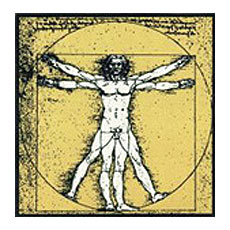
\includegraphics[width=1cm]{img/logoLEO.jpg}
  Scuola Leonardo Da Vinci (Firenze)
}

\author[Stefano Martina]{
  %\\[0.2cm]
  \textbf{Stefano MARTINA}\\
  {\small stefano.martina@gmail.com}
}

\titlegraphic{\tiny
  \href{http://creativecommons.org/licenses/by-sa/4.0/}{
\includegraphics[width=1cm]{img/logoCC.png}}
  This work is licensed under a
  \href{http://creativecommons.org/licenses/by-sa/4.0/}{Creative
    Commons Attribution-ShareAlike 4.0 International License}.}


\title[Lesson 7]{\textbf{Lesson 7 - Pseudocode}}
\date[15/11/15]{\flushright 15 November 2015}

\begin{document}

\begin{frame}[plain]
  \titlepage
\end{frame}

\begin{frame}[fragile]
  \frametitle{Basics}
  \begin{block}{Instructions}
    An \alert{instruction} is a line that ends with a \alert{semicolon}. Some
    instructions can open a \alert{block of code}.
    \begin{cblock}
...;
    \end{cblock}
  \end{block}
  \begin{block}{Code blocks}
    A \alert{block of code} is a series of \alert{instructions} inside a couple of
    curly brackets.
    \begin{cblock}
{
  ...;
  ...;      
  ...;
}
    \end{cblock}
  \end{block}
\end{frame}

\begin{frame}[fragile]
  \frametitle{Program start/end}
  \begin{columns}
    \begin{column}{0.3\textwidth}
      \begin{tikzpicture}
        \node(start) [fStartEnd] {Start};
        \node (dots) [fGeneric, below=of start] {...};
        \node(end) [fStartEnd, below=of dots] {End};
        \draw [arrow] (start) -- (dots);
        \draw [arrow] (dots) -- (end);
      \end{tikzpicture}      
    \end{column}
    \begin{column}{0.7\textwidth}
      \begin{cblock}
{
  variables declarations;
  ...
}
      \end{cblock}
    \end{column}
  \end{columns}
\end{frame}

\begin{frame}[fragile]
  \frametitle{Input}
  \begin{columns}
    \begin{column}{0.4\textwidth}
      \begin{center}
        \begin{tikzpicture}[node distance=5mm, auto]
          \node (start) [fGeneric] {...};
          \node (input) [fInput, below=of start] {variable};
          \node (end) [fGeneric, below=of input] {...};
          \draw [arrow] (start) -- (input);
          \draw [arrow] (input) -- (end);
        \end{tikzpicture}
      \end{center}
    \end{column}
    \begin{column}{0.6\textwidth}
      \begin{cblock}
...
input variable;
...
      \end{cblock}
    \end{column}
  \end{columns}
\end{frame}

\begin{frame}[fragile]
  \frametitle{Output 1}
  \begin{columns}
    \begin{column}{0.4\textwidth}
      \begin{center}
        \begin{tikzpicture}[node distance=5mm, auto]
          \node (start) [fGeneric] {...};
          \node (output) [fOutput, below=of start] {variable};
          \node (end) [fGeneric, below=of output] {...};
          \draw [arrow] (start) -- (output);
          \draw [arrow] (output) -- (end);
        \end{tikzpicture}
      \end{center}
    \end{column}
    \begin{column}{0.6\textwidth}
      \begin{cblock}
...
output variable;
...
      \end{cblock}
    \end{column}
  \end{columns}
\end{frame}
  
\begin{frame}[fragile]
  \frametitle{Output 2}
  \begin{columns}
    \begin{column}{0.4\textwidth}
      \begin{center}
        \begin{tikzpicture}[node distance=5mm, auto]
          \node (start) [fGeneric] {...};
          \node (output) [fOutput, below=of start] {``Text''};
          \node (end) [fGeneric, below=of output] {...};
          \draw [arrow] (start) -- (output);
          \draw [arrow] (output) -- (end);
        \end{tikzpicture}
      \end{center}
    \end{column}
    \begin{column}{0.6\textwidth}
      \begin{cblock}
...
output "Text";
...
      \end{cblock}
    \end{column}
  \end{columns}
\end{frame}

\begin{frame}[fragile]
  \frametitle{Assignation}
  \begin{columns}
    \begin{column}{0.4\textwidth}
      \begin{center}
        \begin{tikzpicture}[node distance=5mm, auto]
          \node (start) [fGeneric] {...};
          \node (ass) [fProcess, below=of start] {variable = ...};
          \node (end) [fGeneric, below=of ass] {...};
          \draw [arrow] (start) -- (ass);
          \draw [arrow] (ass) -- (end);
        \end{tikzpicture}
      \end{center}
    \end{column}
    \begin{column}{0.6\textwidth}
      \begin{cblock}
...
variable = ...;
...
      \end{cblock}
    \end{column}
  \end{columns}
\end{frame}

\begin{frame}[fragile]
  \frametitle{Selection 1}
  \begin{columns}
    \begin{column}{0.4\textwidth}
      \begin{center}
        \begin{tikzpicture}[node distance=5mm, font=\tiny, auto]
          \node(start) [fGeneric] {...};
          \node(selection) [fSelection, below=of start] {Condition};
          \draw [arrow] (start) -- (selection);
          \node(trueBlock) [fGeneric, below=of selection] {true path};
          \draw [arrow] (selection) -- node [near start] {true} (trueBlock);
          \node(falseBlock) [fGeneric, right=10mm of trueBlock] {false path};
          \draw [arrow] (selection) -| node [near start] {false} (falseBlock);
          \node(end) [fGeneric, below=of trueBlock] {...};
          \draw [arrow] (trueBlock) -- (end);
          \draw [arrow] (falseBlock) |- ($ (end.north) + (0,2mm) $);
        \end{tikzpicture}
      \end{center}
    \end{column}
    \begin{column}{0.6\textwidth}
      \begin{cblock}
...
if(condition){
  true path
} else {
  false path
}
...
      \end{cblock}
    \end{column}
  \end{columns}
\end{frame}

\begin{frame}[fragile]
  \frametitle{Selection 2}
  \begin{columns}
    \begin{column}{0.4\textwidth}
      \begin{center}
        \begin{tikzpicture}[node distance=5mm, font=\tiny, auto]
          \node(start) [fGeneric] {...};
          \node(selection) [fSelection, below=of start] {condition};
          \draw [arrow] (start) -- (selection);
          \node(trueBlock) [fGeneric, below=of selection] {true path};
          \draw [arrow] (selection) -- node [near start] {true} (trueBlock);
          \node(end) [fGeneric, below=of trueBlock] {...};
          \draw [arrow] (trueBlock) -- (end);
          \draw [arrow] (selection)
          -- node [near start] {false} ($ (selection.east) + (5mm,0) $)
          |- ($ (end.north) + (0,2mm) $);
        \end{tikzpicture}
      \end{center}  
    \end{column}
    \begin{column}{0.6\textwidth}
      \begin{cblock}
...
if(condition){
  true path
}
...
      \end{cblock}
    \end{column}
  \end{columns}
\end{frame}

\begin{frame}[fragile]
  \frametitle{Selection 3}
  \begin{columns}
    \begin{column}{0.4\textwidth}
      \begin{center}
        \begin{tikzpicture}[node distance=5mm, font=\tiny, auto]
          \node(start) [fGeneric] {...};
          \node(selection) [fSelection, below=of start] {condition};
          \draw [arrow] (start) -- (selection);
          \node(trueBlock) [fGeneric, below=of selection] {false path};
          \draw [arrow] (selection) -- node [near start] {false} (trueBlock);
          \node(end) [fGeneric, below=of trueBlock] {...};
          \draw [arrow] (trueBlock) -- (end);
          \draw [arrow] (selection)
          -- node [near start] {true} ($ (selection.east) + (5mm,0) $)
          |- ($ (end.north) + (0,2mm) $);
        \end{tikzpicture}
      \end{center}  
    \end{column}
    \begin{column}{0.6\textwidth}
      \begin{cblock}
...
if(! condition){
  false path
}
...
      \end{cblock}
    \end{column}
  \end{columns}
\end{frame}

\begin{frame}[fragile]
  \frametitle{Iteration 1}
  \begin{columns}
    \begin{column}{0.4\textwidth}
      \begin{center}
        \begin{tikzpicture}[node distance=5mm, font=\tiny, auto]
          \node(start) [fGeneric] {...};
          \node(selection) [fSelection, below=of start] {condition};
          \draw [arrow] (start) -- (selection);
          \node(iterBlock) [fGeneric, below=of selection] {iteration};
          \draw [arrow] (selection) -- node [near start] {true} (iterBlock);
          \node(end) [fGeneric, below=15mm of iterBlock] {...};
          \draw [arrow] (iterBlock)
          -- ($ (iterBlock.south) - (0,5mm) $)
          -| ($ (selection.west) - (5mm,0) $)
          |- ($ (selection.north) + (0,2.5mm) $);
          \draw [arrow] (selection)
          -- node [near start] {false} ($ (selection.east) + (5mm,0) $)
          |- ($ (end.north) + (0,5mm) $)
          -- (end);
        \end{tikzpicture}
      \end{center}  
    \end{column}
    \begin{column}{0.6\textwidth}
      \begin{cblock}
...
while(condition){
  iteration
}
...
      \end{cblock}
      \begin{block}{Alert}
        If the true and false in the selection are inverted, you need
        to negate the condition like for the \cc{if}.
      \end{block}
    \end{column}
  \end{columns}
\end{frame}

\begin{frame}[fragile]
  \frametitle{Iteration 2}
  \begin{columns}
    \begin{column}{0.4\textwidth}
      \begin{center}
        \begin{tikzpicture}[node distance=5mm, font=\tiny, auto]
          \node(start) [fGeneric] {...};
          \node(iterBlock) [fGeneric, below=of start] {iteration};
          \draw [arrow] (start) -- (iterBlock);
          \node(selection) [fSelection, below=of iterBlock] {condition};
          \draw [arrow] (iterBlock) -- (selection);
          \draw [arrow] (selection) 
          -- node [near start] {true} ($ (selection.west) - (5mm,0) $)
          |- ($ (iterBlock.north) + (0,2.5mm) $);
          \node(end) [fGeneric, below=of selection] {...};
          \draw [arrow] (selection) -- node [near start] {false} (end);
        \end{tikzpicture}
      \end{center}  
    \end{column}
    \begin{column}{0.6\textwidth}
      \begin{cblock}
...
do {
  iteration
} while(condition);
...
      \end{cblock}
      \begin{block}{Alert}
        If the true and false in the selection are inverted, you need
        to negate the condition like for the \cc{if}.
      \end{block}
    \end{column}
  \end{columns}
\end{frame}

\begin{frame}
  \frametitle{Iteration 3}
  \begin{columns}
    \begin{column}{0.33\textwidth}
      \begin{center}
        \begin{tikzpicture}[node distance=5mm, font=\tiny, auto]
          \node(start) [fGeneric] {...};
          \node(iterBlockA) [fGeneric, below=of start] {A};
          \node(selection) [fSelection, below=of iterBlockA] {condition};
          \draw [arrow] (start) -- (iterBlockA);
          \draw [arrow] (iterBlockA) -- (selection);
          \node(iterBlockB) [fGeneric, below=of selection] {B};
          \draw [arrow] (selection) -- node [near start] {true} (iterBlockB);
          \node(end) [fGeneric, below=15mm of iterBlockB] {...};
          \draw [arrow] (iterBlockB)
          -- ($ (iterBlockB.south) - (0,5mm) $)
          -| ($ (selection.west) - (5mm,0) $)
          |- ($ (iterBlockA.north) + (0,2.5mm) $);
          \draw [arrow] (selection)
          -- node [near start] {false} ($ (selection.east) + (5mm,0) $)
          |- ($ (end.north) + (0,5mm) $)
          -- (end);
        \end{tikzpicture}
      \end{center}  
    \end{column}
    \begin{column}{0.33\textwidth}
      \begin{center}
        \begin{tikzpicture}
          \node[arrowNode]{Transforms};
        \end{tikzpicture}
      \end{center}
    \end{column}
    \begin{column}{0.33\textwidth}
      \begin{center}
        \begin{tikzpicture}[node distance=5mm, font=\tiny, auto]
          \node(start) [fGeneric] {...};
          \node(iterBlockA) [fGeneric, below=of start] {A};
          \node(selection) [fSelection, below=of iterBlockA] {condition};
          \draw [arrow] (start) -- (iterBlockA);
          \draw [arrow] (iterBlockA) -- (selection);
          \node(iterBlockB) [fGeneric, below=of selection] {B};
          \draw [arrow] (selection) -- node [near start] {true} (iterBlockB);
          \node(iterBlockA2) [fGeneric, below=of iterBlockB] {A};
          \draw [arrow] (iterBlockB) -- (iterBlockA2);
          \node(end) [fGeneric, below=15mm of iterBlockA2] {...};
          \draw [arrow] (iterBlockA2)
          -- ($ (iterBlockA2.south) - (0,5mm) $)
          -| ($ (selection.west) - (5mm,0) $)
          |- ($ (selection.north) + (0,2.5mm) $);
          \draw [arrow] (selection)
          -- node [near start] {false} ($ (selection.east) + (5mm,0) $)
          |- ($ (end.north) + (0,5mm) $)
          -- (end);
        \end{tikzpicture}
      \end{center}  
    \end{column}
  \end{columns}
\end{frame}

\end{document}
